\section{BDC motor vizsgálata}

%{{{ Szögsebességválasz a névleges feszültségre
\subsection{Szögsebességválasz a névleges feszültségre}

\Aref{subsect:Wu-w}. részfeladatban meghatározott átviteli függvényt fogjuk megvizsgálni.
A bemenőjel
\begin{equation}
	\fn{X} = \frac{\un}{s},
\end{equation}
ez az egységugrás függvény Laplace-transzformáltja felnagyítva a névleges feszültségre.
A kimenőjel Laplace-transzformáltja
\begin{equation}
	\fn{Y} = \fn{W}_{\fn{U}_0\rightarrow\Omega_\text{ki}}\fn{X} = \frac{\km }{\La\Ja s^2 + \Ja\Ra s + \ke\km}\frac{\un}{s}
\end{equation}

Ezt invez Laplace-transzformálva megkapjuk a szögsebesség válasz időfüggvényét:
\begin{equation}
	\fn{y}(t) = \mathcal{L}^{-1}(\fn{Y}) = 
	618.34 - 618.34\, \mathrm{e}^{- 3651.3\, t}\, \left(\cosh\!\left(3582.2\, t\right) + 1.0193\, \sinh\!\left(3582.2\, t\right)\right)
\end{equation}
amit \aref{fig:2-a}. ábra mutat.

\begin{figure}[H]
	\centering
	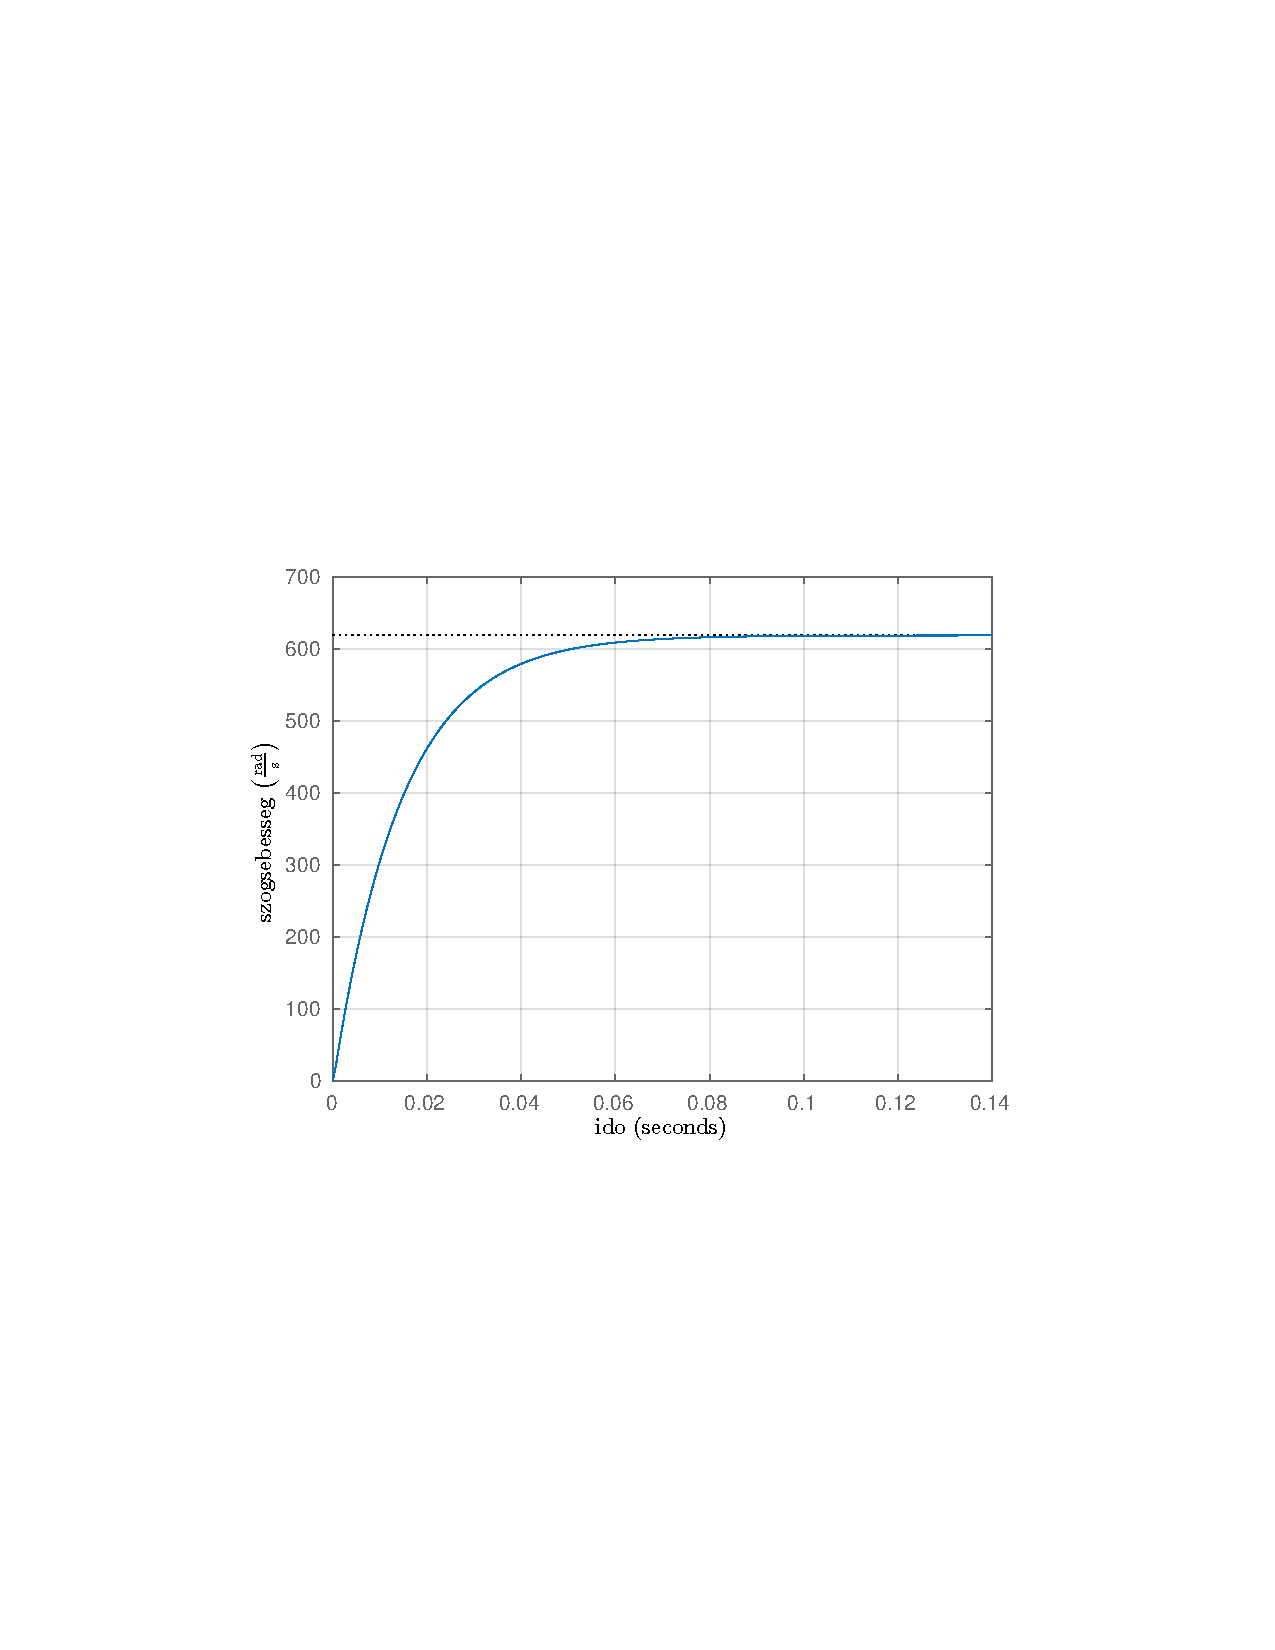
\includegraphics[width=.8\textwidth, trim=110 245 110 272, clip]{2-a}
	\caption{Szögsebesség válasz a névleges feszültségre}
	\label{fig:2-a}
\end{figure}

A kezdeti és az állandósult szögsebesség a végérték tételek segítségével számolható:
\begin{equation}
	\omega(0) = \lim\limits_{s\rightarrow \infty}s\fn{Y} = 0~\frac{\text{rad}}{\text{s}}
\end{equation}
\begin{equation}
	\omega(\infty) = \lim\limits_{s\rightarrow 0}s\fn{Y} = 618,34~\frac{\text{rad}}{\text{s}}
\end{equation}

A motor adatlapja a terhelés nélküli szögsebességet 5860 rpm = 613.66 $\frac{\text{rad}}{\text{s}}$-nek adja meg. A számított 0.76 \%-os relatív hiba numerikus hibáknak tudható be.

%}}}

%{{{ Áram kimenet a névleges feszültség hatására
\subsection{Áram kimenet a névleges feszültség hatására}

\Aref{subsect:Wu-i}. részfeladatban meghatározott átviteli függvényt fogjuk megvizsgálni.
%
A kimenőjel Laplace-transzformáltja
\begin{equation}
	\fn{Y} = \fn{W}_{\fn{U}_0\rightarrow \fn{I}_\text{a}}\fn{X} = \frac{\km }{\La\Ja s^2 + \Ja\Ra s + \ke\km}\frac{\un}{s}
\end{equation}

Ezt invez Laplace-transzformálva megkapjuk a szögsebesség válasz időfüggvényét:
\begin{equation}
	\fn{y}(t) = \mathcal{L}^{-1}(\fn{Y}) = 
	3.3058\, \mathrm{e}^{- 69.098\, t} - 3.3058\, \mathrm{e}^{- 7233.5\, t}
\end{equation}
amit \aref{fig:2-b}. ábra mutat.

\begin{figure}[H]
	\centering
	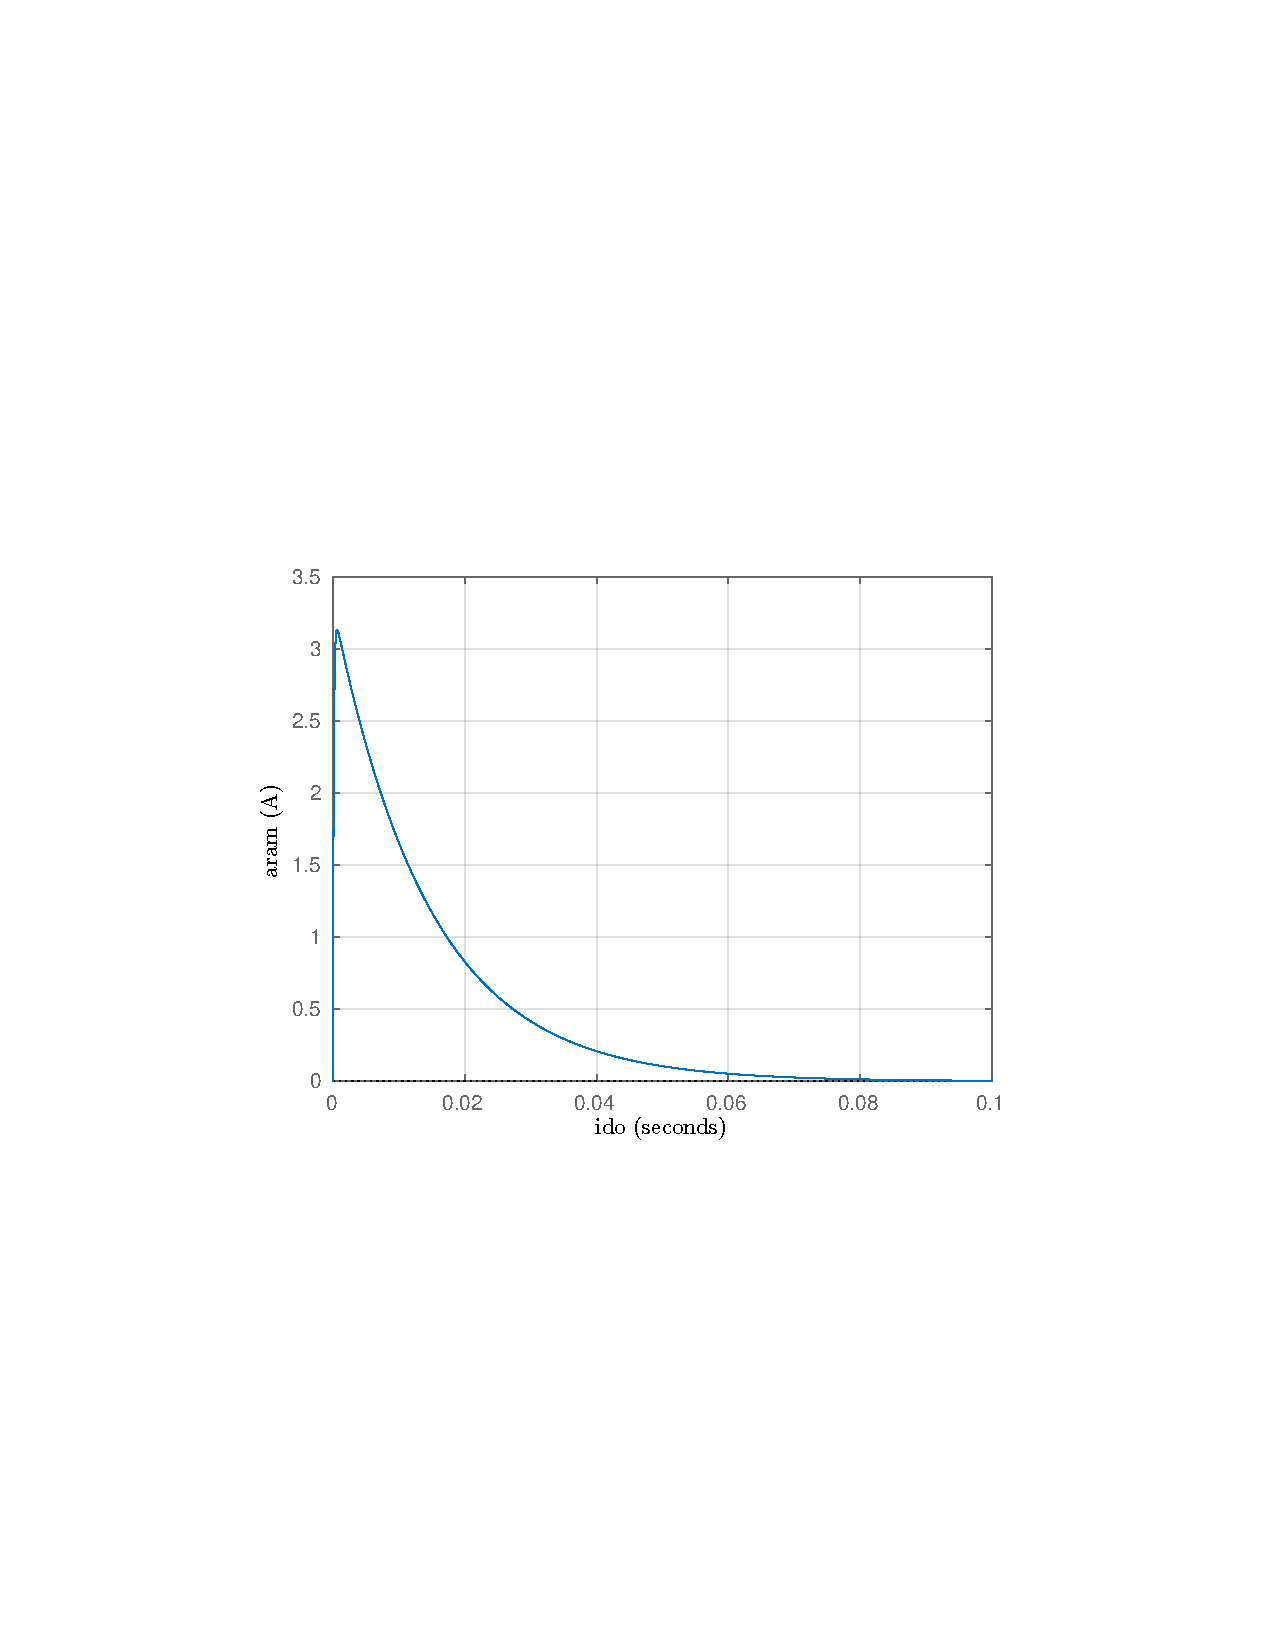
\includegraphics[width=.8\textwidth, trim=110 245 110 272, clip]{2-b}
	\caption{Áram kimenet a névleges feszültség hatására}
	\label{fig:2-b}
\end{figure}

A kezdeti és az állandósult áram a végérték tételek segítségével számolható:
\begin{equation}
	\fn{I}_\text{a}(0) = \lim\limits_{s\rightarrow \infty}s\fn{Y} = 0\text{ A}
\end{equation}
\begin{equation}
	\fn{I}_\text{a}(\infty) = \lim\limits_{s\rightarrow 0}s\fn{Y} = 0\text{ A}
\end{equation}

%}}}

%{{{ Nyomaték kimenet a névleges feszültség hatására
\subsection{Nyomaték kimenet a névleges feszültség hatására}

A DC motor egyenletei alapján
\begin{equation}
	\tau_\text{v} = \km \fn{I}_\text{a}
\end{equation}

A kimenőjel időfüggvénye:
\begin{equation}
	\fn{y}(t) = \km \fn{y}_{\fn{I}_\text{a}}(t) =
	0.18911\, \mathrm{e}^{- 6.9145\, t} - 0.18911\, \mathrm{e}^{- 7295.7\, t}
\end{equation}
amit \aref{fig:2-c}. ábra mutat.

\begin{figure}[H]
	\centering
	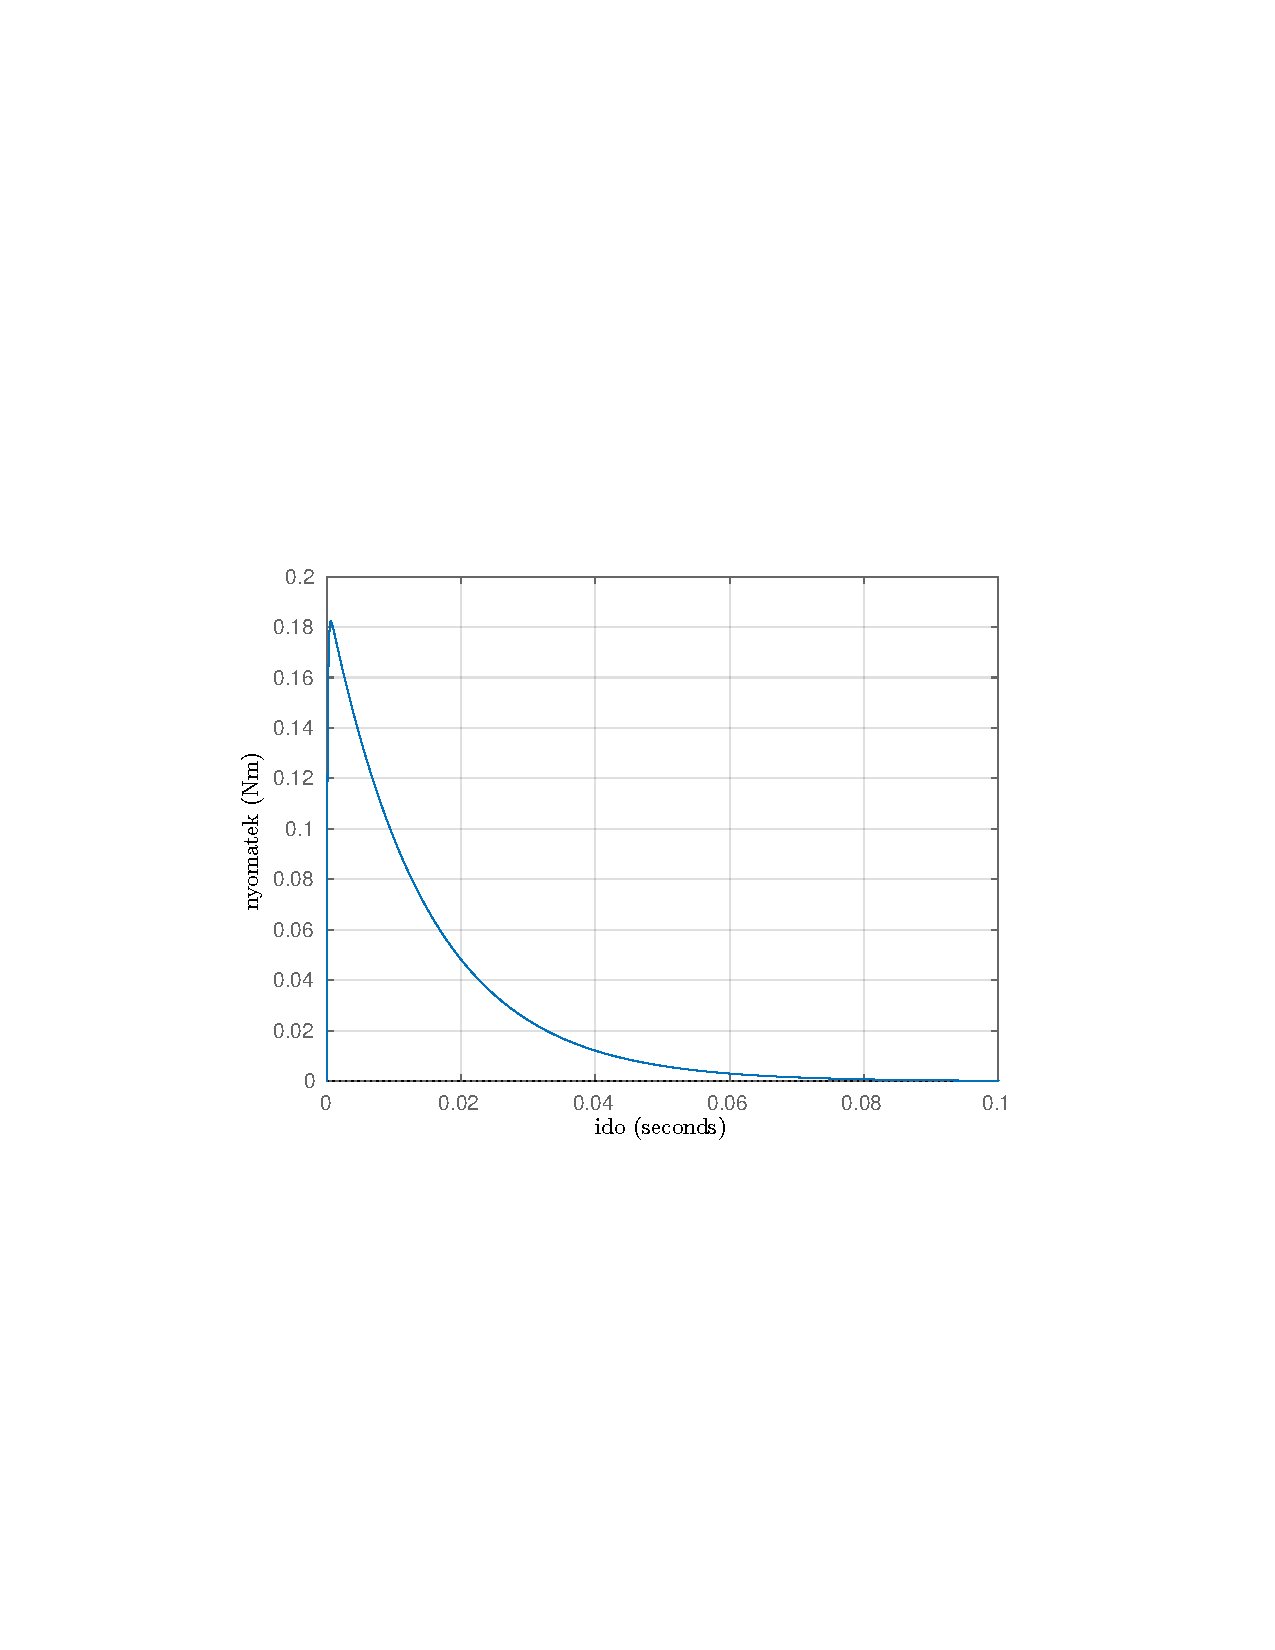
\includegraphics[width=.8\textwidth, trim=110 245 110 272, clip]{2-c}
	\caption{Nyomaték kimenet a névleges feszültség hatására}
	\label{fig:2-c}
\end{figure}

A kezdeti és az állandósult nyomaték analóg módon számolható:
\begin{equation}
	\tau_\text{v}(0) = \km 0\text{ A} = 0\text{ Nm}
\end{equation}
\begin{equation}
	\tau_\text{v}(\infty) = \km 0\text{ A} = 0\text{ Nm}
\end{equation}

%}}}
